%proofread!

\documentclass[draft,jgrga]{agutex}
\usepackage[dvips]{graphicx}
\usepackage{amsmath}
\usepackage{multirow}

\usepackage{tabularx}
%\usepackage{lineno}
%\linenumbers*[1]

%\noindent $>$latex file \\
%\noindent $>$dvips -P pdf -o file.ps file.dvi \\
%\noindent $>$ps2pdf13 file.ps file.pdf

\authorrunninghead{GUTOWSKI ET AL.}
\titlerunninghead{Radar uncertainty}

\authoraddr{D. Blankenship, Institute for Geophysics, University of Texas at Austin}
\authoraddr{Gail Gutowski, Department of Geosceinces, University of Texas at Austin (gail.gutowski@utexas.edu)}
\authoraddr{Charles S. Jackson, Institute for Geophysics, University of Texas at Austin}
\authoraddr{Duncan Young,  Institute for Geophysics, University of Texas at Austin}

\begin{document}

\title{Uncertainty of ice-penetrating radar and corresponding uncertainty at Byrd Ice Core, Antartica}



\begin{abstract}
%Data from radar-sounding surveys of West Antarctica are used to determine the age of observed radar horizons near the Byrd ice core, Antarctica~\citep{gow1968}. We emphasize inclusion of uncertainty in radar- and ice-related sources of uncertainty. The analysis is based on a basic ice-flow model developed by~\citet{schwander2001}. The model assumes no basal melting, zero velocity at the bed, and linear strain rate below 1200 meters depth.

%A Bayesian uncertainty analysis is performed to reduce uncertainties and make the best use of the available data. The analysis quantifies observational limitations of the analysis, informing future uncertainty reduction through refinement of observational techniques. A Research Plan outlines a Bayesian approach to develop a new chronology of the Byrd ice core which takes into account theoretical and measurement uncertainties in depth and age of prominent layers observed in the ice column. The method employs Markov Chain Monte Carlo modeling to invert for accumulation and strain as functions of depth.


%Our goal is to determine the uncertainty in age and depth of observed radar reflection horizons near Byrd Station, West Antarctica through comparison with the Byrd ice core record. Here we show the distribution of age and depth with their modeled uncertainties based on the methods described above.  

%We determine the uncertainty in comparing age-depth relationships from ice core records to 




Ice-penetrating radar (IPR) is a useful tool for investigating past and present climatic conditions and developing a better understanding of ice dynamics.  Interpretation of the data for the purpose of  climate or ice dynamics studies requires accurate dating of internal radar reflection horizons. This can be achieved through the combination of IPR and age-depth profiles established from ice cores. To do so, it is therefore necessary to consider contributions to uncertainty from both aircraft-based IPR data and ice-core dating techniques. The Airborne Geophysical Survey of the Amundsen Sea Embayment (AGASEA) project has provided a wealth of focused IPR data for West Antarctica. We consider uncertainty due to phase selection and bandwidth in ten bright radar horizons observed near Byrd Station, West Antarctica to determine the depth range from which each of the horizons originates. We use a simplified ice flow model to transfer an age-depth relationship for the Byrd ice core to the radar horizons using a Bayesian inversion method. The inversion considers uncertainty in the ice core dates to determine model parameters. A new ensemble of age-depth profiles for Byrd Station is then obtained through forward modeling of the inverted model parameters.






 but interpretation and analysis of the data requires an understanding of the uncertainty introduced by aircraft-based IPR. 

%ADD: \\
%       where did accum come from?\\
%	comparison to Morley flow?
%	discussion of layers/age deeper in the ice sheet
%	add more numbers/tables;\\
%5	fill out who? references;\\
%	add plenty of references\
%	add bibtex references
%	further description of schwander model?;\\
%	future work
%	discussion of correlation between layers
%	discussion of wa-wa
%	discussion of ECM?
%	where did sd's on age come from? -- NOT 3percent!;\\
%	proofread\\
%	fix figures \\


\end{abstract}

\begin{article}
\section{Introduction}

Understanding ice dynamics and mass balance of ice sheets is important to predict how the Earth�s polar regions will respond to global environmental change. While studies of mountain glaciers strongly suggest significant ice depletion in the next century given current global warming trends (cite: someone from Fairbanks), the response of large-scale ice sheets such as Greenland and Antarctica is uncertain. This is largely due to a lack of information about the internal dynamics of these ice sheets.

Greenland and Antarctica represent a disproportionate potential contribution to sea level rise; the two major ice sheets contain enough ice to raise sea levels by XX m, while all mountain glaciers combined contain only XX m of potential sea level rise (cite). Because of this, it is essential that we get a firm grasp on how these massive ice sheets respond to climate change. 

One approach to this problem is to examine how ice sheets have respond to changes in climatic conditions in the past. Age-depth relationships from ice cores have historically been used as a tool for understanding ice dynamics and accumulation history in particular points of an ice sheet (Cite: someone who provides chronology of ice core). More recently, ice-penetrating radar has been combined with the ice core data to extend age-depth profiles over larger regions of the ice sheet (cite: Neumann 2008, others)

Ice-penetrating radar surveys of ice sheets are a glimpse into the ice sheet, providing an opportunity to spatially extend age-depth information determined at an ice core site. Because internal radar horizons encode information about accumulation rates and ice deformation, they can be used to develop a picture of ice dynamics. This information is particularly useful for dynamical ice sheet modeling efforts currently underway (cite some dynamical modeling efforts?).

However, in order to be incorporated into ice sheet models, it is first important to understand the uncertainty in the ice-penetrating radar data. The accuracy of dating internal radar horizons depends on the uncertainty in the radar observations themselves and the uncertainty in ice-core dating. \cite{eisen2004} evaluated this uncertainty for ground-based radar in the top 100 m of the East Antarctic Ice Sheet. We approach the problem using airborne observations of WAIS near Byrd ice core and consider radar horizons in the top 1300 m of the ice sheet.  We use an ice-core derived chronology and a one-dimensional ice flow model to evaluate the uncertainty in airborne ice-penetrating radar observations. We present a resulting ensemble of age-depth profiles, which includes appropriate consideration of the uncertainties involved in the derivation.

\section{Data}

\subsection{Radar Data}
Radar reflection horizons provide an avenue for developing an understanding of ice dynamics. Each year, snow accumulates on the surface of the ice sheet. The physical properties of this snow contain information about climatic conditions at the time of deposition; for instance, the oxygen isotope$\delta^{18}O$ can be used as a proxy for temperature. Over time, the surface layer is covered with the accumulation of subsequent years and becomes buried in the ice column. Differences in chemical composition of these deposited layers lead to variations in electrical conductivity observed by the radar as horizons, or horizontal layers. We therefore interpret the radar horizons as isochronous \citet{eisen2004}.

Ice-penetrating radar-echo sounding data was obtained in December 2004 as part of the Airborne Geophysical Survey of the Amundsen Sea Embayment (AGASEA) project \citep{holt2006}. The radar line passed 870 m from the Byrd ice core site while the plane was travelling 67 m/s at an elevation of 550 m above the ice surface. The data includes two-way travel times (the time it takes for a radar pulse to be transmitted, reflect off a layer, and return to the receiver) in microseconds, which were collected with a 15 MHz bandwidth. We use ten strong radar horizons that were hand-traced at the University of Texas Institute for Geophysics using the seismic imaging software \textit{GeoFrame}. The horizons were selected for their prominence, which ensured that they could be traced through the domain.

\subsection{Byrd ice core chronology}

The Byrd ice core was drilled in 1968 and was the first in Antarctica to extend to bedrock \citep{gow1968}. Damage to the ice core above 88 m prohibited the traditional approach of annual layer counting, so the chronology was instead determined by locating the 1259 AD volcanic horizon at 97.8 m below the 1968 ice surface. Below 88 m, the electrical conductivity method (ECM) was used to date the ice core \citep{hammer1994}. The ECM method measures variations in electrical conductivity. Between 300 m and 900 m, brittle ice precluded sufficient ECM measurements. \citet{hammer1994} instead fit the chronology with three piecewise linear functions. The resulting layer-thickness profile was integrated from surface to depth to obtain an age-depth relationship for the length of the ice core.

\citet{hammer1997} presented a volcanic chronology based on this previously derived timescale in which volcanic events were matched to peaks in electrical conductivity. The chronology includes dated volcanic events that cover an age range from 709 BP to more than 18000 BP, corresponding to depths ranging from 97.8 m to 1890 m below the 1968 surface of the Byrd ice core.

Ice density data as a function of depth were obtained from the original analysis of the ice core \citep{gow1968}. The data were used to account for the varying density of ice in the upper part of the ice sheet. The result was used to apply a constant firn correction to the ice thickness at Byrd ice core. 

\section{Sources of Uncertainty}\label{unc}
There are many sources of uncertainty inherent to the way in which
data is collected, analyzed, and understood. We have included the
following sources of uncertainty.

\subsection{Radar Uncertainty}

Radar horizons, surfaces of constant two-way travel time (TWTT), are hand-traced using seismic interpretation software. This allows a user to select strong reflectors from a radargram and trace them along a radar line. However, there is a limit to the accuracy of tracking a single phase of a radar reflection. The vertical accuracy depends on the resolution of the sampling rate of the radar transmitter as well as considerations of noise. For high sampling rates, the uncertainty in phase selection is typically $\frac{\lambda}{4}$, but can be as accurate as $\frac{\lambda}{2}$ for data with high signal-to-noise where $\lambda$ is the wavelength of the electromagnetic pulse.  The sampling rate for the data used here varies from 5 ns to 20 ns. To be conservative, we assume a 10 ns resolution when tracking the phase of reflections from the surface of the ice sheet and from each internal layer. We treat the surface and internal layers separately in this instance. 

To convert TWTT uncertainty into units of depth, we scale the time by the velocity of electromagnetic wave propagation in the medium. The pulse travelled from the aircraft to the ice sheet surface with velocity, c, the speed of light, and then slowed to the velocity of electromagnetic wave propagation in ice, which we take to be $\textit{c}_i$ = 1.69 x 10$^8$ m/s before reaching the internal layers and reflecting back. The corresponding 1$\sigma$ uncertainty is $\sigma_{surf}$ $\sim$0.3 m for the surface reflector and $\sigma_{lay}~\sim~$0.17 m for each of the internal layers, assuming the uncertainty is gaussian.
 
The uncertainty associated with picking the elevation of the surface is considered a systematic error because the same surface elevation will be used to normalize all of the internal layers. The TWTT uncertainty of each of the internal layers is applied randomly because each of the individual layers need not have the same uncertainty. This is because the reflection from each layer need not have the same phase with respect to the sampling rate. To account for this, we assume the TWTT to be normally distributed and sample randomly from this distribution for each of the internal layers independently.

The finite bandwidth of the data means that even an infinitesimally thin layer of ice will appear in the survey to have a finite width. Our data uses a pulse bandwidth of 15 MHz. This translates to a 1$\sigma$ depth uncertainty of 5.63 m, obtained from considering both the bandwidth frequency and the velocity of electromagnetic radiation in ice. This uncertainty is applied as a random, normally distributed error in the depth of each of our selected layers. 




\subsection{Age Uncertainty}\label{ageunc}

%Each year fresh snow accumulates on the top of the ice sheet,
%burying the previous season's snowfall. As layers of ice descend into
%the ice sheet, the layers become thinner, as air from the surface is
%squeezed out and gravity compacts the ice. This thinning makes it
%increasingly difficult to distinguish one layer from another at
%depth while in shallow regions, it maybe be possible to simply count
%layers by eye and therefore determine the age of those layers. 

%The uncertainty associated with determining ages for ice layers is a
%function of depth;
%-delta age \\
%-landmarks like 10Be, CH4, F \\
%-ecm method accuracy \\
%-correlation with bc89? \\


Each year, fresh snow accumulates on top of the ice sheet, burying the previous season?s snowfall. As layers of ice descend into the ice sheet, they become thinner because air is squeezed out and gravity compacts the ice. This thinning makes it increasingly difficult to distinguish one layer from another at depth. In shallow regions, it is possible to count layers by eye to determine the age of near-surface isochrones; however, this is harder to do deep in the ice sheet.
The uncertainty associated with determining ages for ice layers is therefore a function of depth. 

%Several sources are responsible for increased uncertainty with depth. There are %two methods of dating ice cores: by ice age or by gas age \citep{bender2006}. %This is because ice in the upper part of the glacier still contains atmospheric %gases until such a depth as pore closure occurs, cutting off the connection %between ice at depth and the atmosphere. Because the air is able to penetrate %below the surface and into the firn layer, ice at a given depth tends to be %older than the air at that depth. This discrepancy leads to an ambiguity in the %true age of the ice if atmospheric chemistry is used to determine the age of %the ice. 

The upper part of the original 1968 Byrd ice core was too damaged to count annual layers. However, in 1989, a shallow core dubbed NBY89 was drilled nearby which enabled \citep{langway1994} to complete a chronology for the top 164 m of the core. Using the ECM method \footnote{ The Electrical Conductivity Method (ECM) is another approach to dating ice. It involves measuring the conductivity of ice at different depths \citep{hammer1994}. This conductivity is associated with the composition of the ice, characterized by its acidity level. Layers of ash embedded in the ice, for example, will have a distinct conductivity. The ECM method is particularly useful in deep parts of the ice column where it is difficult to otherwise distinguish isochronous layers due to layer thinning.}, they matched 3 volcanic events to the original ice core with an uncertainty of $\sigma_{age} = \pm$ 2 yr for the upper 1360 a of the ice core.

Isotopic dating is common among ice core chronologies. Landmark events for concentrations of Beryllium-10, methane, and fluorine (to name a few) are matched to chemical analyses of the ice \citep{schwander2001} at different points in time. Accepted dates for these events are then mapped onto the ice core. 

We adopt the following estimates of uncertainty to accompany the isotopic dating, though no comprehensive review of uncertainty from these methods is available. The end of the Younger Dryas period is correlated between the GRIP and Byrd ice cores using CH$_4$. This method indicates an uncertainty of roughly $\sigma_{age} = \pm$ 150 yr for the period between 1360 a and 11.5 ka \citep{ blunier1998, schwander2001}. This incorporates uncertainty in the $\delta$age estimate on the GRIP and Byrd cores ($\pm$ 100 yr) as well as the CH$_4$ match between the GRIP/Byrd ($\pm$ 100 yr). For the period between 11500 a and 17320, we adopt an uncertainty of $\sigma_{age} = \pm$ 300 yr \citep{schwander2001}. This value is the result of stratigraphic layer counting near a prominent fluoride peak at Byrd station, tuned by matching CH$_4$ during the Younger Dryas period.

For layers older than 17320 a, we assume $\sigma_{age}$ = 2 ka based on U/Th dating of the Laschamp geomagnetic excursion \citep{schramm2000}. Note that we include this uncertainty for completeness; the ten radar horizons of interest in this analysis are believed to be younger than 17320 a.

Table~\ref{age_unc} summarizes the uncertainty we assign to observed ages as a function of depth.





\section{Method}\label{method}

We use an ice flow model adapted from \citet{morland2009} to determine the age of internal layers near the Byrd ice core drilling site in Antarctica.  The simple flow model has the following form:
\begin{equation}
\frac{\overline{z}}{h_0} = \frac{1}{1-r} [1 - exp(-s \overline{t}]
\overline{z} = h_0 - z
r = \frac{b}{q}
s = s_ds_0
\end{equation}

where depth, $\overline{z}$ is defined to be 0 at the base, $h_0 =$ 2164 m is the depth at the ice sheet surface, b is basal melting rate, q is the accumulation rate, and $\overline{t}$ is the age corresponding to $\overline{z}$. The optimum constant strain rate, $\textit{s}$, is used to achieve reasonable correlations between the model and observations; $s_0$ is the initial strain rate and $s_d=$0.722 for the Byrd ice core. The model assumes isostatic equilibrium, constant ice density, uniform strain rate in $\textit{z}$, and $\textit{r}$ $<$ 1 (i.e. nonnegative mass balance in the ice column). Note that it is difficult to know accumulation rate on its own due to layer thinning within the ice column. As such, we consider layer thickness instead of layer accumulation because it can be physically measured using the techniques described previously. Further, while depth in the model, $\overline{z}$, is defined so that $\overline{z}$(base) $=$ 0, the following analysis is discussed in terms of depth $\textit{z}$, where $\textit{z(surface)} = 0$.

We use the flow model to invert for layer thickness as a function of depth, $\textit{q}$, and strain scale factor, $\textit{s}$, using an observed age-depth relationship. We use the resulting parameters to evaluate the age of ten prominent radar horizons. The inversion is done using a Markov Chain Monte Carlo technique known as the Metropolis. We use a stepwise function to describe layer thickness, breaking it into four depth regimes:

\[
z = 
\begin{cases}
z1 & \text{for} < 150 \text{m} \\
z2 & \text{for} \ge 150 \text{ m and} < \text{1024 m} \\
z3 & \text{for} \ge 1024 \text{m and} < 1294 \text{m} \\
z4 & \text{for} \ge 1292 \text{m}
\end{cases}
\]

These regimes were chosen based on a linear piecewise function of layer thickness developed by \citet{hammer1994} in which shifts are seen at the above transition points.

The Metropolis algorithm utilizes prior knowledge about the model parameters (accumulation and strain scale factor) to develop a joint posterior distribution of the parameters. We use truncated uniform priors on all parameters, allowing them to take on values within a physically reasonable range: layer thickness is allowed to vary between 0 cm/a and 30 cm/a, while the strain scale factor may take values between 0 and 1.7.  The model is initialized using random parameter values within these ranges.

At each model step, we evaluate the age model at every point in the ice column based on proposed sets of parameters.  An associated cost is calculated as a measure of the model/data misfit for each proposal. The log likelihood is described in equation~\ref{cost}:

\begin{equation}\label{cost}
log likelihood = \frac{(Age_{model}~ - ~Age_{obs})^2}{(\sigma_{obs})^2}
\end{equation}

where $Age_{model}$ is evalation of the \citet{morland2009} ice flow model for a given accumulation and strain scale factor. $Age_{obs}$ and $\sigma_{obs}$ come from the volcanic age-depth function and we allow for the aforementioned uncertainty in $Age_{obs}$ (see Table~\ref{age_unc})to loosen the constraint on the cost function. At each iteration the algorithm makes a decision about whether or not to accept the combination of parameters based on the cost: if the cost of the $\textit{n}$th iteration is less than the cost of the $\textit{(n-1)}$th iteration, the set of parameters is accepted. This means that the $\textit{n}$th set of parameters is a better fit to the data, because the cost has decreased. If the cost of the current nth iteration is greater than the cost of the $\textit{(n-1)}$th iteration, the set of parameters is accepted with probability $exp[-\frac{cost_n~-~cost_{n-1}}{2}]$, the Metropolis probability. The algorithm continues on a random walk through parameter space, minimizing cost at each step.

We use the Metropolis algorithm to generate a large number of age-depth distributions that together describe the probability of the age of a radar horizon at a given depth based on knowledge about ice flow and layer thickness. We generate 20000 sets of parameters (accumulation and strain rate) that characterize physically reasonable models of age-depth. Age uncertainty is taken to be the variance in age at a given depth. 

Uncertainty in the radar-derived depth of each horizon is considered next. To find the radar sampling rate uncertainties, we draw a single value from the probability distribution for the surface reflector, described by $\sigma_{surf}$. We then randomly sample ten values from a probability distribution described by $\sigma_{lay}$, resulting in a radar sampling rate for each of the horizons of interest. The bandwidth uncertainty is found in the same fashion as the sampling rate error for the layers. The bandwidth and sampling rate uncertainty vectors are summed in quadrature to arrive at a total radar uncertainty for each radar horizon. We also add a correction for firn density and account for additional accumulation between 1968 (when the core was drilled) and 2004 (when the radar line was flown) assuming a constant accumulation rate of 11 cm/a \cite{hammer1994}. 

This process is repeated 20000 times to build a probability distribution describing the depth of each radar horizon. For each sample in depth probability distribution (20000 in all), we randomly sample an age-depth model from the ensemble generated previously. The selected model is evaluated at each of the ten radar horizon depths for a given sample. The result is an ensemble of 20000 age-depth profiles for the radar horizons of interest which incorporate uncertainty in both age and depth.



\section{Results}


Figure~\ref{depthhist} shows the distribution of modeled depths associated with each ice layer of interest from radar observations near Byrd Station, West Antarctica. The spread in the distribution is indicative of uncertainty due to observational methods. Table~$\ref{results}$ shows the standard deviation of depth for each of the ten chosen layers, assuming the errors to be gaussian. See Section~$\ref{ageunc}$ for a full discussion of the sources of uncertainty included in this analysis. The uncertainty in each layer depth is more or less constant with depth. However, deeper in the ice sheet, near X m and Xm,  multiple radar horizons observed as being distinct are consistent within uncertainty with being from the same source. 

The corresponding age distributions are shown in Figure~\ref{agehist} and again assume gaussian errors. Table~\ref{results} shows the mean and standard deviation for each peak. Due to increased uncertainty in ice core dating, age uncertainty increases with depth. As with depth, layers at X m and X m are consistent with originating during the same period. This ambiguity makes it clear that robust uncertainty quantification is critical for the interpretation of internal layers; dynamic analyses require that radar horizons be distinguished in order to obtain a time-dependent profile of ice flow. 

Figure~$\ref{spaghetti}$ shows an ensemble of modeled age-depth distributions for the ten picked radar layers. The distributions are trained on the observed volcanic record at Byrd Station, allowing for uncertainties in both depth and age. Note that both systematic and random sources of uncertainty are included. Crossing lines indicate that random uncertainty plays a significant part in the age-depth distribution of ice layers at Byrd Station. Spread between ensembles that do not cross is representative of systematic uncertainties in the model. 

As described in Section~$\ref{method}$, the model is based on five parameters: layer thickness parameters in four depth regimes and a ratio of surface to bed ice velocity. Figure~$\ref{accum}$ shows the distributions of the layer thickness parameters, which are used as a proxy for accumulation in the model. As expected due to layer thinning with depth, mean layer thickness decreases with depth. The modeled layer thickness is consistent with layer thickness at the Western Divide determined by \citep{neumann2008} above 1294 m; Table~\ref{accums} shows a comparison between the two. We expect layer thickness to be at a maximum at the divide and therefore reasonable values at Byrd Station should be less than those at the divide. Our modeled layer thickness below 1294 m is larger than shallower modeled thicknesses and greatly exceeds the layer thickness at the divide at this depth. However, this depth corresponds to only the deepest radar horizon of interest, so it should not affect the result.

\section{Discussion and Conclusion}
Uncertainty associated with two-way travel time in airborne ice-penetrating radar surveys of Antarctica is not thoroughly understood. We seek to quantify that uncertainty and its affect on depth and age uncertainties near Byrd Station, West Antarctica. Our approach employs a simple ice flow model and basic parameter assumptions which we will improve upon in the future. The ice flow model used in this analysis relies heavily on the function of ice accumulation chosen. Here we have chosen to simplify our approach by using layer thickness as a proxy for accumulation. By proposing constant layer thickness in each of four depth regimes, we further approximate accumulation with a discontinuous function. Our depth regimes were selected based on an approximation by \citet{hammer1994}. While a useful tool, a continuous function of accumulation will be included in the future.

Another assumption in our analysis is the choice of ice flow model. We use a simple model developed for the Byrd ice core by \citet{morland2009}. To further simplify the model, we assume no basal melting, however this is a poor assumption based on the amount of liquid water found at the base of the icee sheet when the core was drilled to bedrock \citep{gow1968}. Geothermal flux derived from a borehole temperature profile was estimated to be 75 mW m$^-2$ by \citet{gow1968}. Additionally, the model assumes only vertical strain, ignoring potentially important longitudinal contributions to ice flow. Ice near Byrd Station is flowing at $v_{surf}$ $\sim$ 11 m/a, about 0.5 km since the Byrd ice core was drilled, so it is important to include horizontal components in future analyses \citep{bindschadler1997}. The wide-ranging nature of continuous radar observations make radar data ideal for studying these kinds of longitudinal effects, which will be included with more complex models of ice flow in the future.

%to include:
%layer thickness not as good as accumulation -- overestimating, perhaps problem with %discontinuities
%allow for correlation between layers
%future: include comparison on models (likelihood functions) for comparison

\section{Draft notes}
%1. Emphasize that radar uncertainties are for nadir and doesn't account for side reflections? \\
%2. Other/different/prettier figures?\\
2. Include map of ice core and flight path/radar data location
%3. Draw a schematic of Metropolis algorithm (r.v. interdependence)?\\
4. What does overestimation of layer thickness (and therefore accum) indicate about the model?\\
%5. Include plot of power to match layers?
%5. Discussion: How to reduce uncertainties?
%6. Include plot of strain scale factor?


\bibliographystyle{agu}
\bibliography{bib}
\end{article}

%Figures

\begin{figure}
\centering
	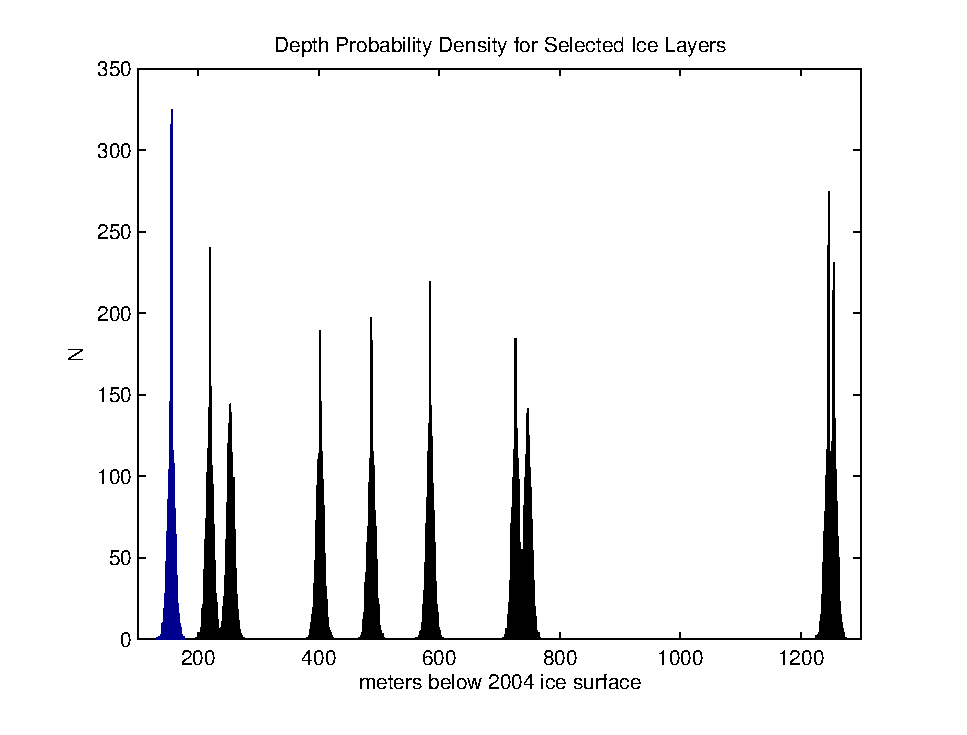
\includegraphics[scale=0.6]{depthhist_morland.eps}
	\label{depthhist}
	\caption{Histogram of modeled water-equivalent ice depth for each of ten apparently prominent layers observed using airborne radar near Byrd Station, West Antarctica. The width of each distribution is the result of uncertainties arising from the method of radar collection, as discussed in Section~$\ref{method}$.}
\end{figure}

\begin{figure}
	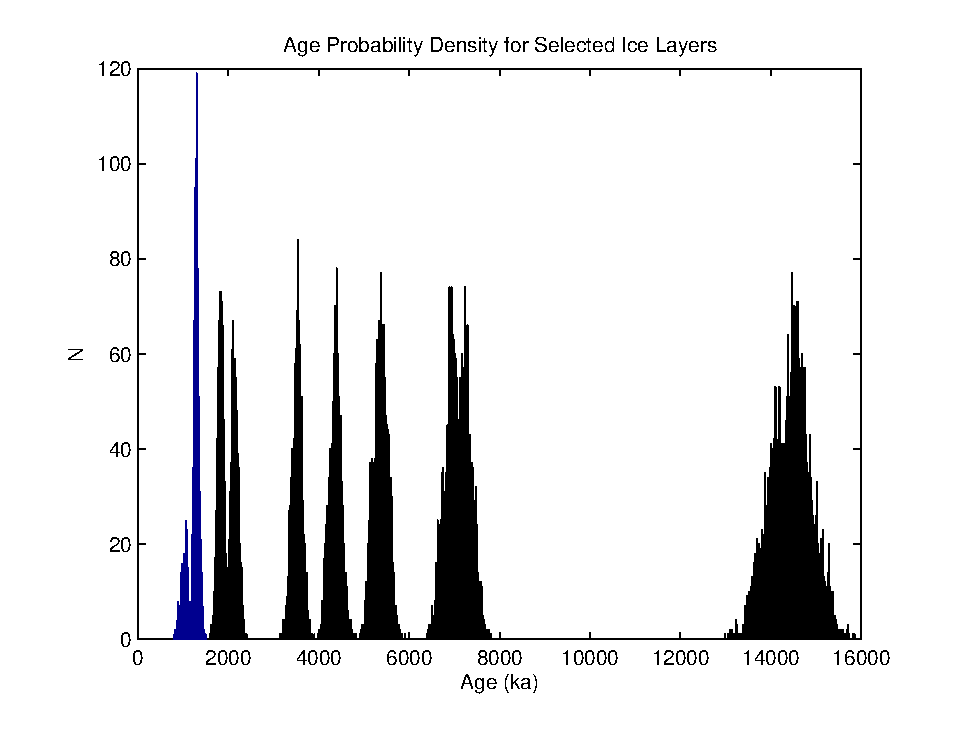
\includegraphics[scale=0.6]{agehist_morland.eps}
	\label{agehist}
	\caption{Histogram of the age distribution for each of ten prominent layers observed using airborne radar near Byrd Station, West Antarctica. The distribution of ages associated with each layer represents the uncertainty in assigning ages to layers at varying depths. Age uncertainty stems from both radar uncertainty and isotopic ice core dating uncertainties.}
\end{figure}

\begin{figure}
	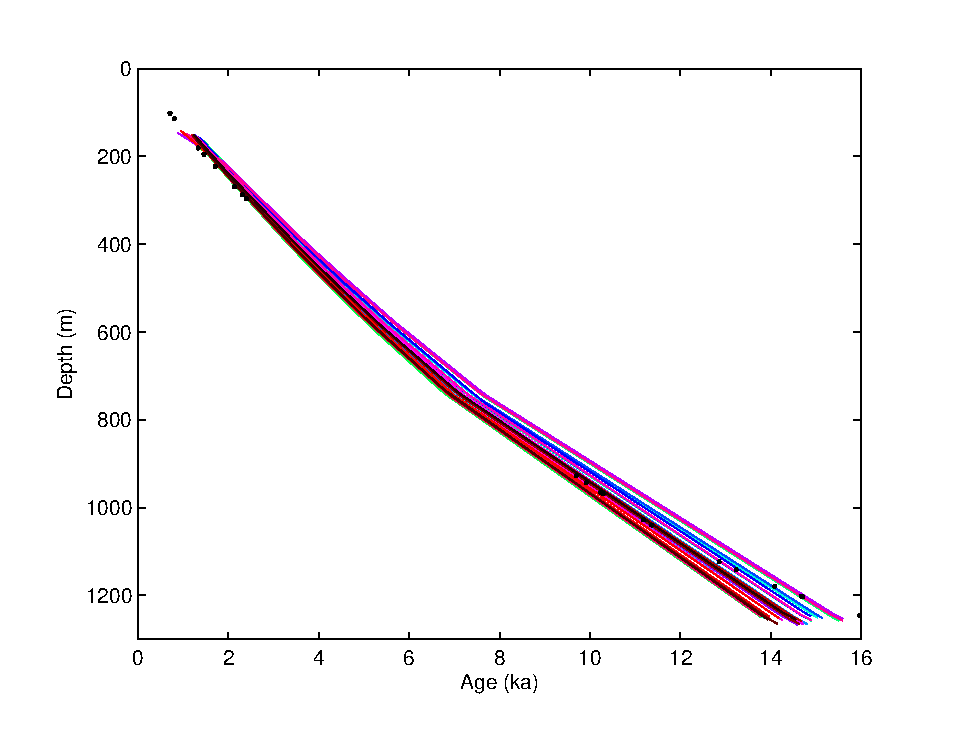
\includegraphics[scale=0.6]{spaghetti_morland.eps}
	\label{spaghetti}
	\caption{ Modeled age-depth distribution of layers observed using airborne radar near Byrd Station, West Antarctica. Black dots represent isotopically-dated volcanic events from the ice core record at Byrd Station. Each line represents a set of parameters (see Section~$\ref{method}$~that describe the observed data within uncertainty.    }
\end{figure}


%\begin{figure}
%	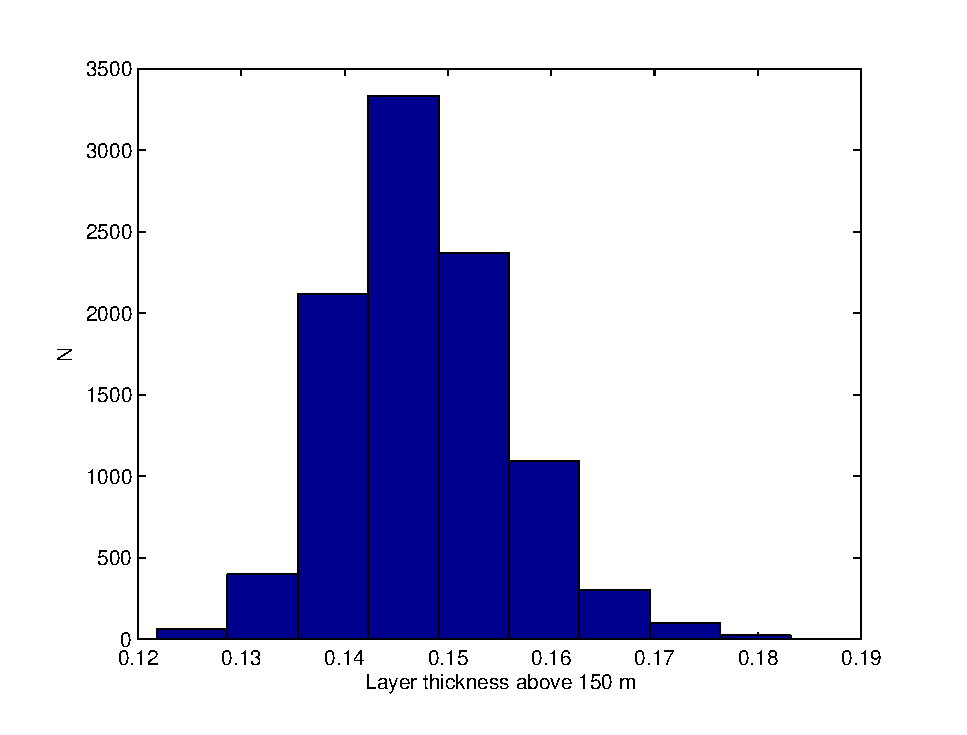
\includegraphics{thickgt150.eps}
%	\label{accum}
%	\caption{Modeled layer thickness in each of four depth regimes near Byrd Station, West Antarctica. **Check what observed is in each of these regimes to compare to mean of distribs** }
%\end{figure}
%\begin{figure}
%	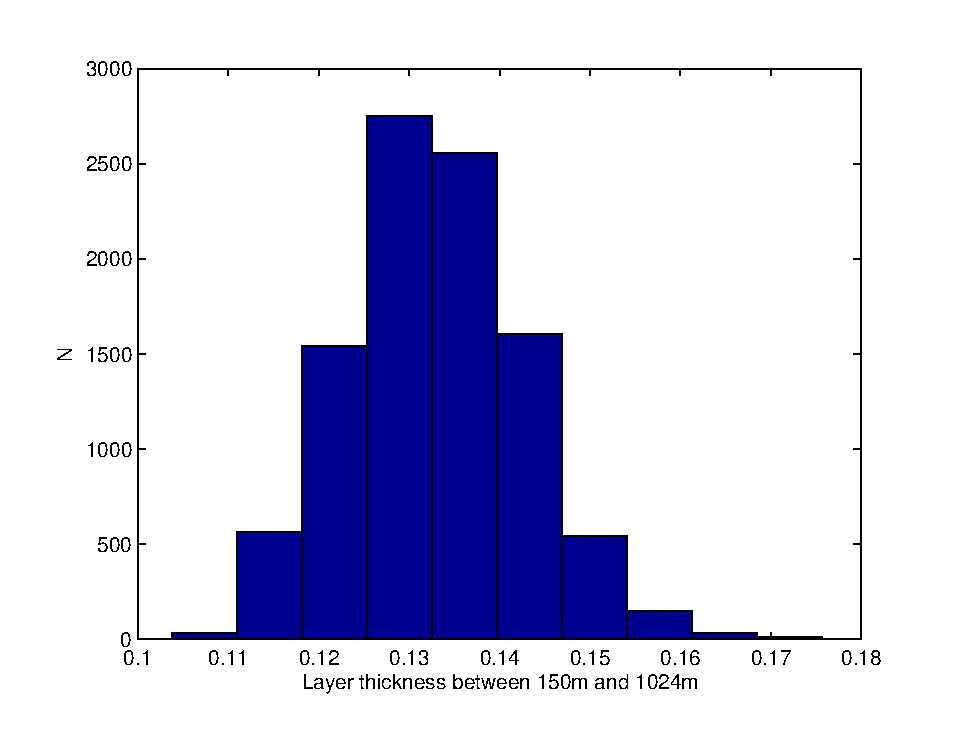
\includegraphics{thickgt1024lt150.eps}
%	\label{accum}
%	\caption{Modeled layer thickness in each of four depth regimes near Byrd Station, West Antarctica. **Check what observed is in each of these regimes to compare to mean of distribs** }
%\end{figure}
%\begin{figure}
%	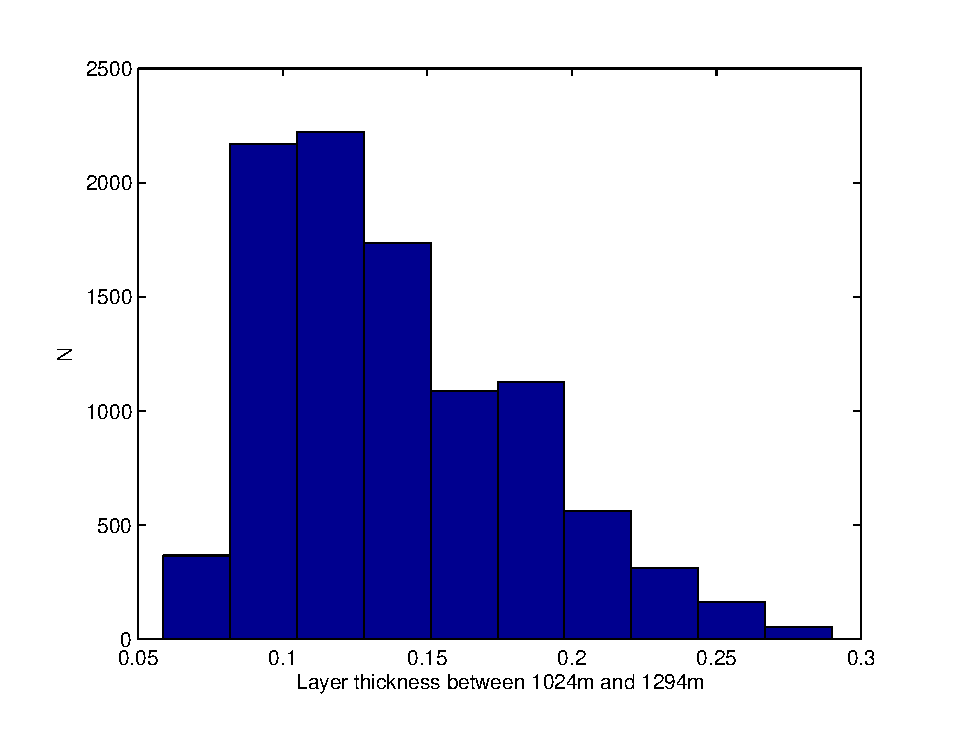
\includegraphics{thickgt1294lt150.eps}
%	\label{accum}
%	\caption{Modeled layer thickness in each of four depth regimes near Byrd Station, West Antarctica. **Check what observed is in each of these regimes to compare to mean of distribs** }
%\end{figure}
%\begin{figure}
%	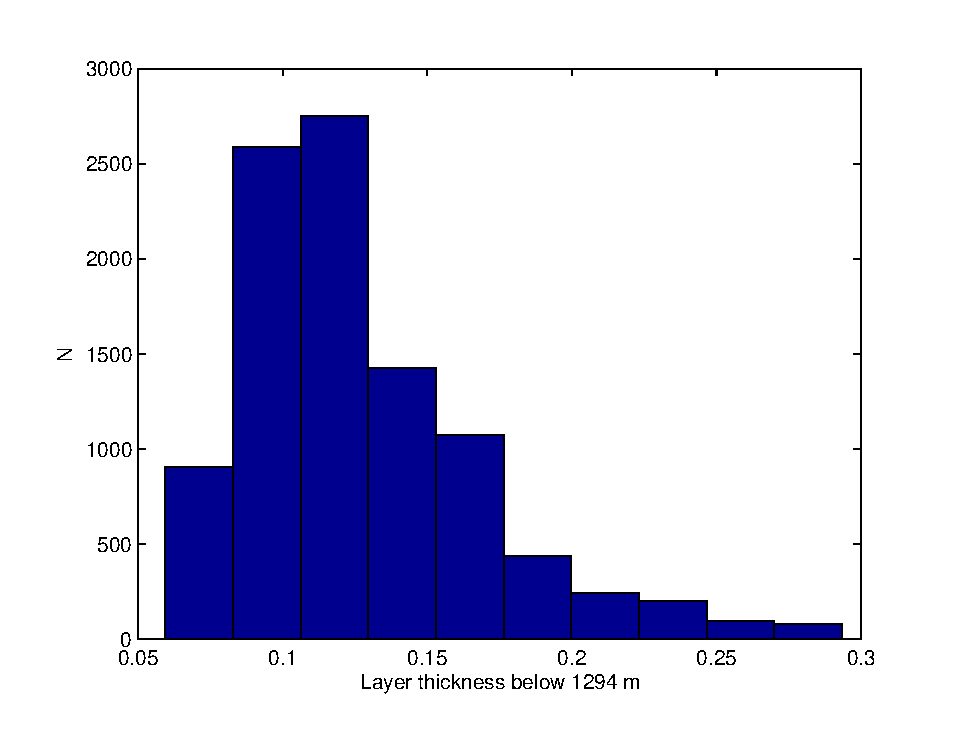
\includegraphics{thickgt1294.eps}
%	\label{accum}
%	\caption{Modeled layer thickness in each of four depth regimes near Byrd Station, West Antarctica. **Check what observed is in each of these regimes to compare to mean of distribs** }
%\end{figure}

\begin{figure}\label{accum}
\begin{center}$
\begin{array}{cc}
\includegraphics[width=2.5in]{laythick.eps}
%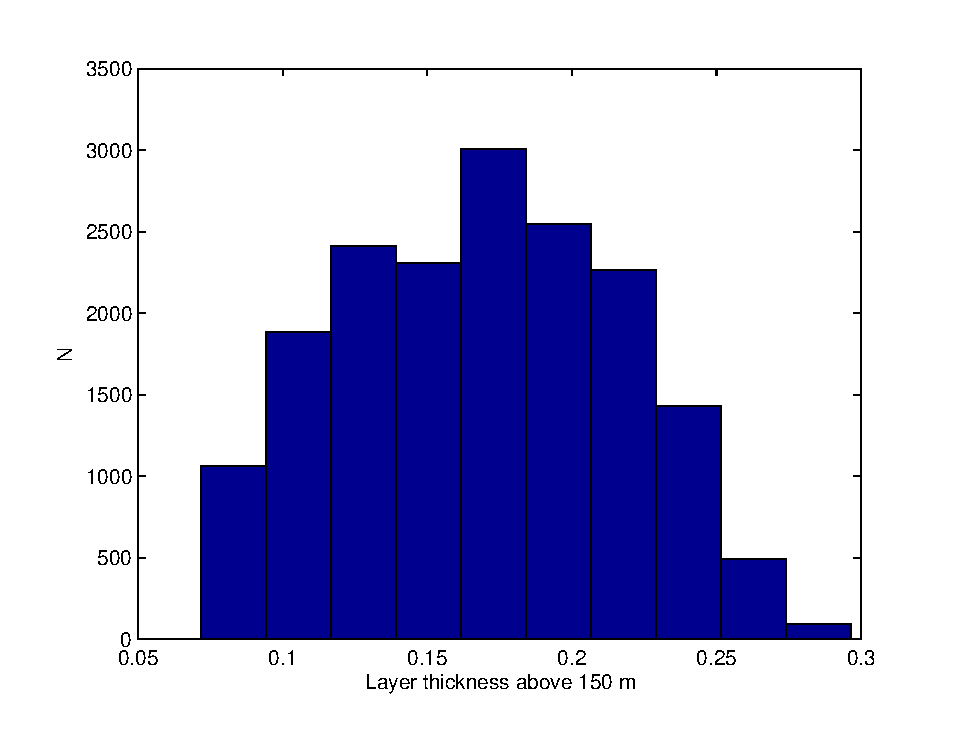
\includegraphics[width=2.5in]{thicklt150_morland.eps} &
%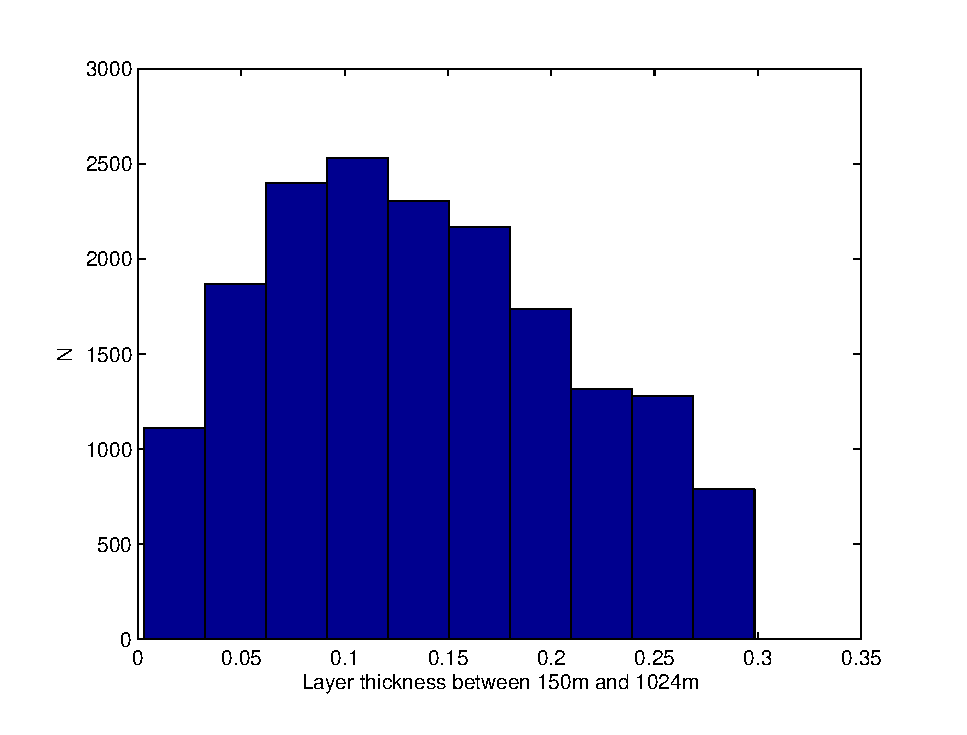
\includegraphics[width=2.5in]{thickgt150lt1024_morland.eps} \\ 
%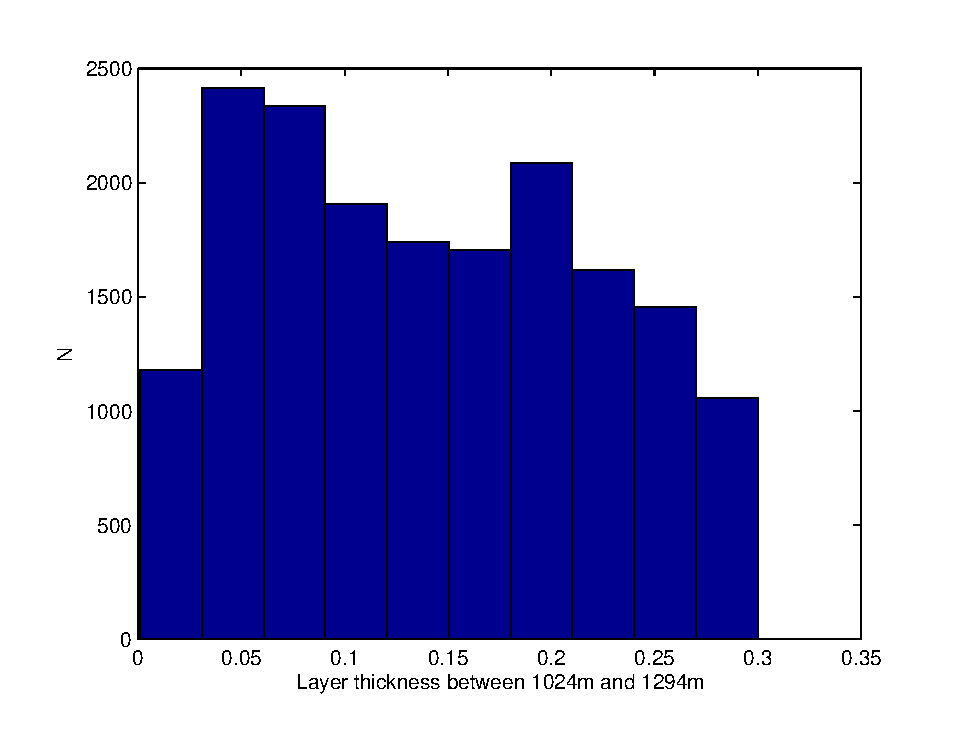
\includegraphics[width=2.5in]{thickgt1024lt1294_morland.eps} &
%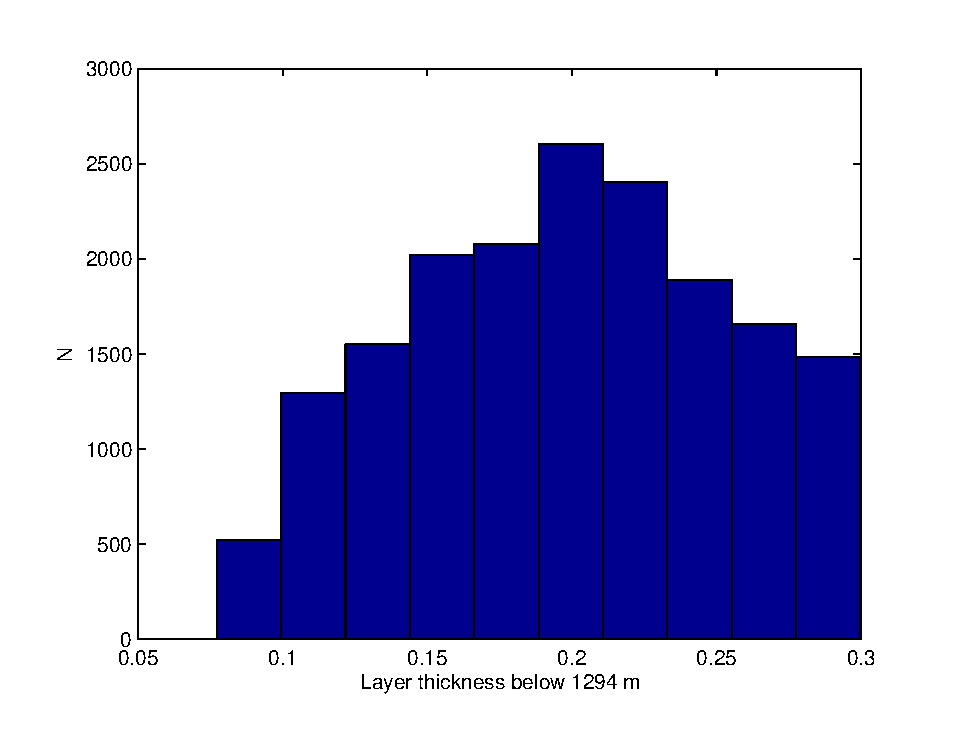
\includegraphics[width=2.5in]{thickgt1294_morland.eps}
\end{array}$
\end{center}
\caption{Modeled layer thickness in each of four depth regimes near Byrd Station, West Antarctica. The model overestimates layer thickness, particulary in deeper regimes. }
\end{figure}


\begin{table}\label{accums}
\caption{Comparison between layer thickness at the Western Divide between the Ross and Amundson Seas \citep{neumann2008} and modeled here at Byrd Station. Maximum layer thickness occurs at the divide, so layer thicknesses at Byrd Station are expected to be less, but comparable, at Byrd Station.}
\begin{tabular}{|c|c|c}
\hline
Depth Range (m) & Layer thickness at Divide (m/a) & Layer thickness at Byrd (m/a) & 1$\sigma$ Uncertainty  \\
\hline
d $<$ 150 & $\sim$0.27 & $\sim$ 0.18 \\
150 $<$ d $<$ 1024 & $\sim$ 0.14 - 0.27 &   & \\
1024 $<$ d $<$ 1294 & $\sim$ 0.08 - 0.14 &  & \\
d $>$ 1294& $<$ 0.08 &  0.20 & \\
\hline
\end{tabular}
\end{table}

\begin{table}\label{age_unc}
\caption{Uncertainty in ice core dates based on analysis by \citet{schwander2001} for Dome C, Antarctica. Age uncertainty is considered to be gaussian with standard deviation from a variety of age reference points.}
\begin{tabular}{|p{4cm}|p{4cm}|p{8cm}|}
\hline
 Age (a) & 1$\sigma$ Uncertainty (a) & Method of Dating  \\
\hline
&&\\
Age $<$ 1360 & $\pm$ 2  & ECM method on a shallow follow-up ice core, NBY89 from \citep{langway1994}\\
& & \\
1360 $\ge$ Age $>$ 11500 & $\pm$ 150  & end of Younger Dryas period and $^{10}Be$ peak ]\citetp{blunier98} \\
&& \\
11500 $\ge$ Age $>$ 17320 & $\pm$ 300 & significant volcanic event "Old Faithful" from \citet{hammer1994}\\
&&\\
Age $\ge$ 17320 & $\pm$ 2000 & U/Th dating of Laschamp geomagnatic excursion \citep{schramm2000}\\
\hline
\end{tabular}
%\tablenotetext{a}{Footnote text here.}
\end{table}



\begin{table}\label{results}
\caption{Depth and age mean, median, and uncertainty for ten strong radar reflectors near Byrd Station, West Antarctica. The radar two-way travel time (TWTT) is given in column 1. }
\centering
\begin{tabular}{| l || l | l | c || c | c | c |}
\hline
\multirow{2}{*}{TWTT (us)} &  \multicolumn{3}{c||}{Depth (m)} & \multicolumn{3}{c|}{Age (a)} \\   
\cline{2-7}
 & Mean & Median & Std Dev & Mean & Median & Std Dev \\
\hline
 6.02   & 167.6  & 167.6  & 1.178 & 1204. & 1203. & 10   \\
 6.775  & 231.4  & 231.4  & 1.182 & 1793. & 1791. & 20   \\
 7.18   & 265.6  & 265.6  & 1.165 & 2095. & 2096. & 28  \\
 8.94   & 414.4  & 414.4  & 1.183 & 3505. & 3512. & 70   \\
 9.9402 & 499.6  & 499.6  & 1.178 & 4385. & 4397. & 95   \\
 11.1   & 596.9  & 596.9  & 1.183 & 5443. & 5462. & 126   \\
 12.78  & 738.8  & 738.8  & 1.178 & 7096. & 7126. & 175   \\
 13.02  & 759.1  & 759.1  & 1.172 & 7354. & 7386. & 183   \\
 18.92  & 1257.7 & 1257.7 & 1.177 & 15828. & 15631. & 838   \\
 19.0205 & 1266.2 & 1266.2 & 1.178 & 15990. & 15785. & 868  \\
\hline
\end{tabular}
%\tablenotetext{a}{Footnote text here.}
\end{table}

\end{document}

